\newpage
\section{Fault-Tolerance Design}
\label{sec:ftDesign}
This section describes the design of the archive service in case of different kinds of failures. The system being part of a large Distributed system,
faces different difficult situation which must be handled for a stable application. Table \ref{table:probServices} lists the possible errors which 
could occur with a brief description i.e. network issues, failure of a 
dependent service, sudden termination of the archive service. 
\begin{longtable}{|p{4cm}|p{10cm}|}
    \hline
        \textbf{Errors}  & \textbf{Description}\\
    \hline
        Network glitches & The MARS framework is built upon a complex distributed architecture and the communication between the services
        happen via a network (e.g HTTP, RPC). It is a possibility that the connection cannot be established for a small period of time due to network problems.
        This would lead the archive service to fail even though all the services are functioning.\\
    \hline
        Failure of a dependent service & There is a possibility that a service which the archive service is dependent upon goes down temporarily due to an unexpected
        failure or is in maintenance. The failure of the dependent service to reply would also generate an error in the Archive service.\\
    \hline
        Sudden failure of the Archive service & Like all the other services the Archive service is also prone to getting an unexpected restart. This restart would cause
        the running job to stop and the progress to be lost.\\    
    \hline
    \caption{Possible errors which could occur in the Archive service}
    \label{table:probServices} 
\end{longtable}

Figure \ref{fig:activityFailure} illustrates the activity diagram which describes how the Archive service will be designed so that a recovery from errors mentioned in
Table \ref{table:probServices} could be handled. The main strategy for the failure mitigation is to re-run the process again from the beginning once an error occurs. 
The number of restarts and wait time can be configured by a programmer. This is designed in such a way so that the service avoids a deadlock situation of the
resource being restarted infinitely. Additionally, a cumulative wait time for the restart can also be added so that there is some gap between the process restart.

\begin{figure}[H]
    \centering 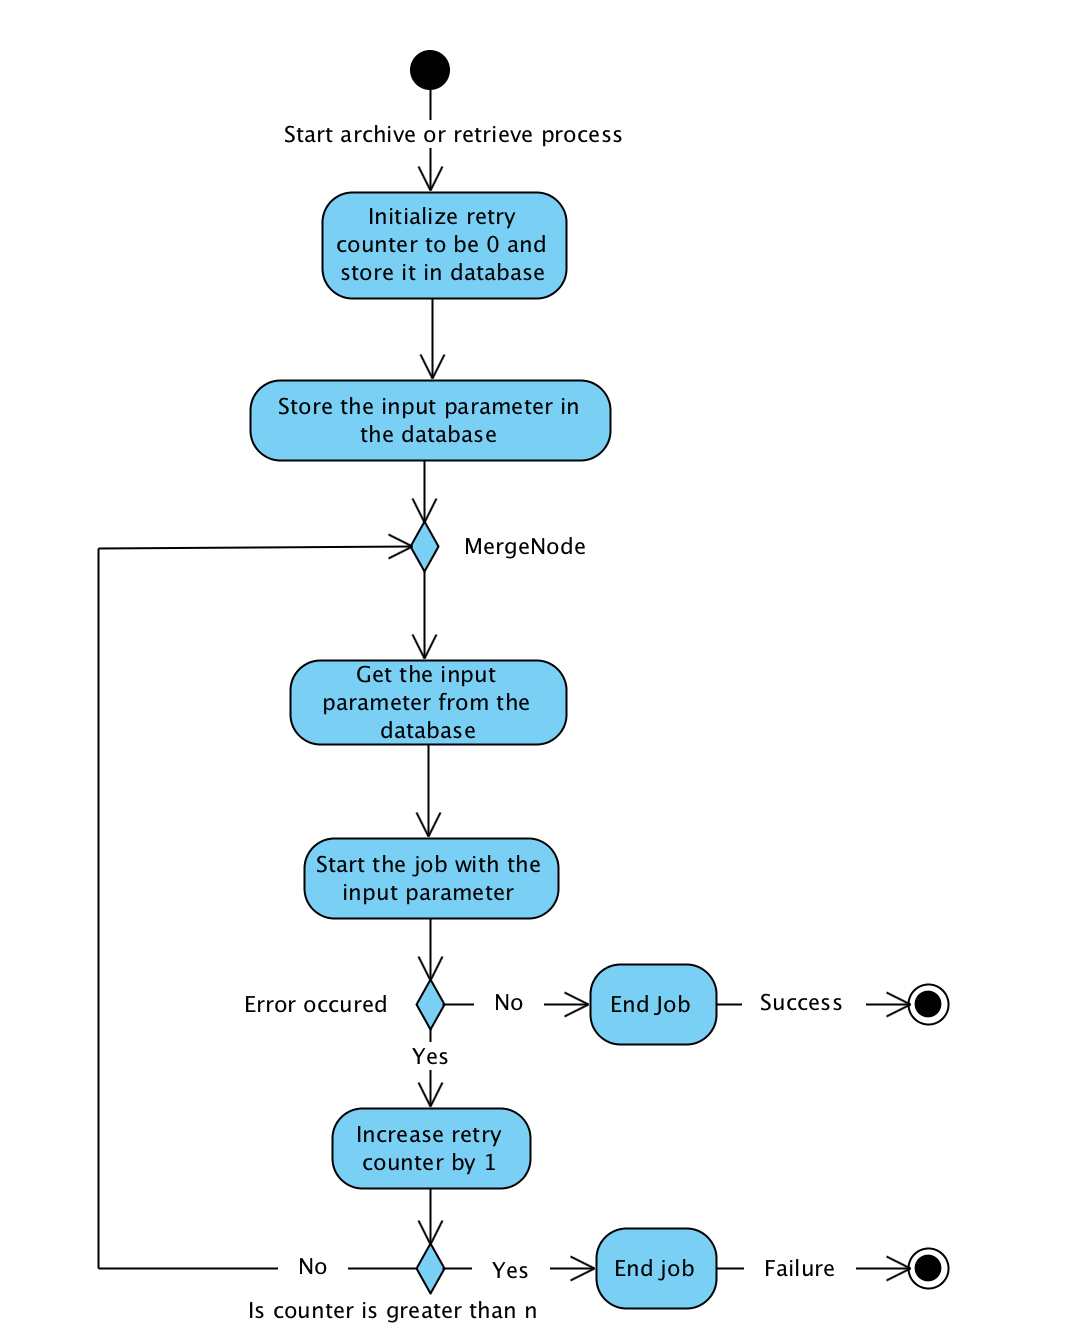
\includegraphics[scale=0.6]{grafiken/activityFailure.png}
    \caption{Activity Diagram for failure mitigation for the Archive service}
    \label{fig:activityFailure}
\end{figure}
